\section{Fuzzy Inference}

\subsection{Determining Fuzzy sets}

As mentioned in the previous section, the noises in the image inevitably introduces uncertainties to our system. Therefore the feature values referenced in our rules have to be represented in fuzzy sets.

To determine the \textbf{best fuzzy sets capturing the appropriate degree of uncertainties}, we use the statistics from the training data to find the optimal threshold.

For $Thinness$, we use 3 fuzzy sets for ellipse-like, rectangle-like and triangle-like $Extent$ ratio. For $Extent$, we use 2 fuzzy sets for circle-like and square-like $Thinness$ ratio. The shapes and boundries of these fuzzy sets are determined based on the \textbf{distribution of feature values in the training data and their 25-th, 75-th and extreme percentiles}. The final fuzzy sets are illustrated in Figure 3 and Figure 4 (Figures not drawn to scale).

%\begin{figure}[ht!]
%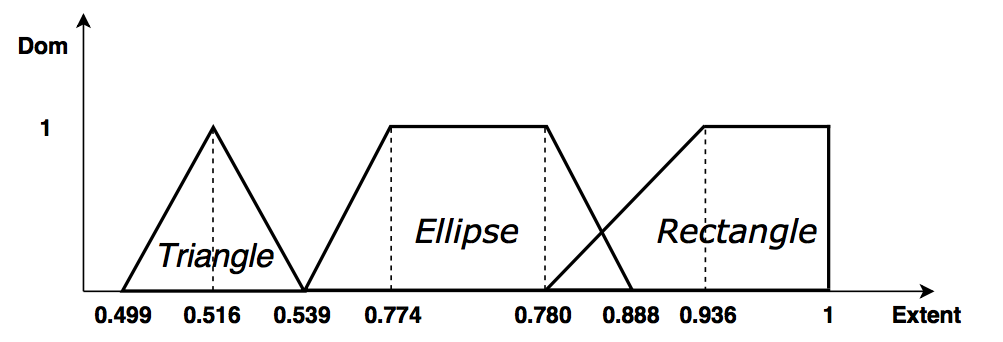
\includegraphics[width=.5\columnwidth]{Figure_3_Fuzzy_Sets_1.png}
%\caption{Fuzzy Set of Extent}
%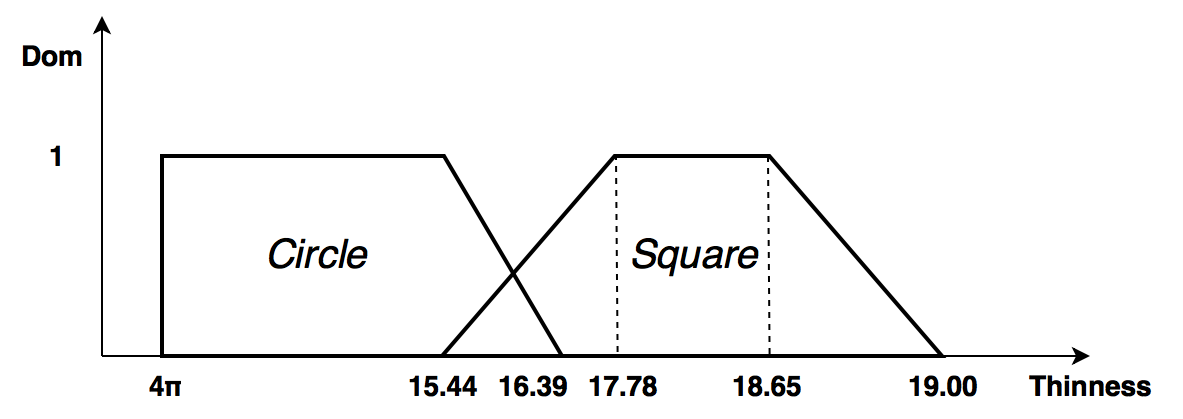
\includegraphics[width=.5\columnwidth]{Figure_4_Fuzzy_Sets_2.png}
%\caption{Fuzzy Set of Thinness}
%\end{figure}

\begin{figure}

\begin{subfigure}[b]{\columnwidth}
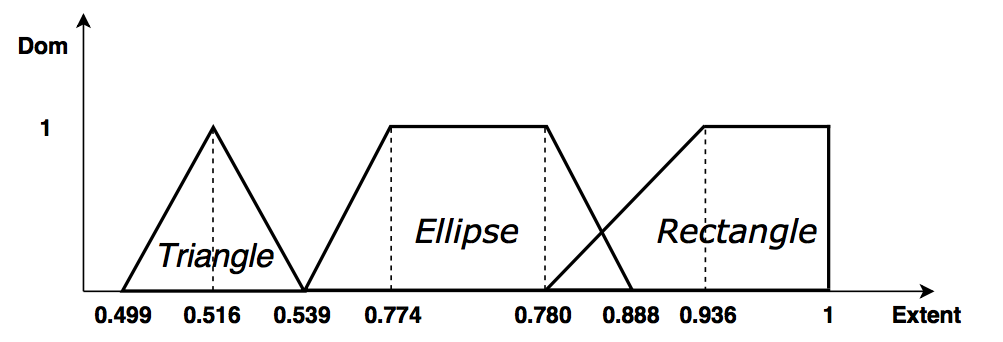
\includegraphics[width=\columnwidth]{Figure_3_Fuzzy_Sets_1.png}
\caption{Fuzzy Set of Extent}\end{subfigure}

\begin{subfigure}[b]{\columnwidth}
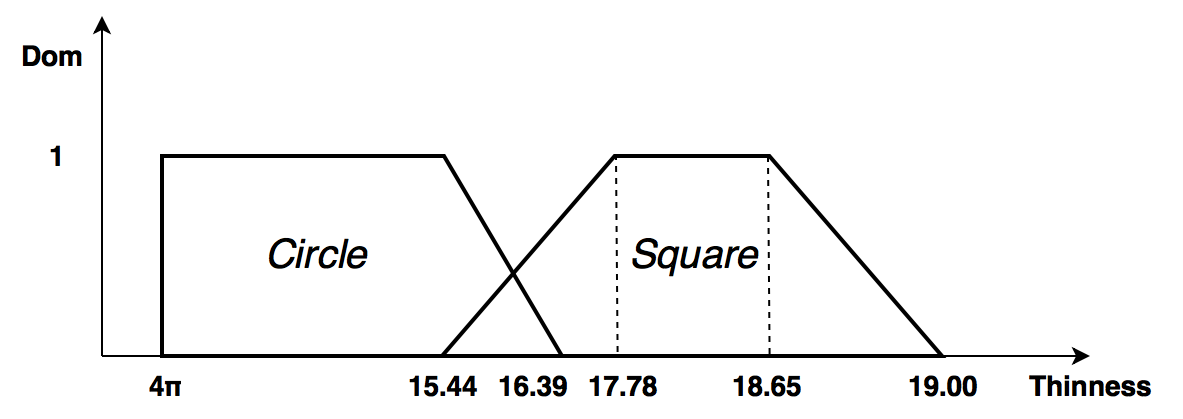
\includegraphics[width=\columnwidth]{Figure_4_Fuzzy_Sets_2.png}
\caption{Fuzzy Set of Thinness}
\end{subfigure}

\end{figure}

\subsection{Implementing Inference Engine}

Now that the fuzzy sets are determined, we have to implement the inference engine. However, the specific nature of our task requires us to make some adaptations to the the usual fuzzy inference engine.

Firstly, unlike the example from the textbook, the set of possible outputs in our task is \textbf{not} a set of linguistic values which can be represented by a series of contiguous intervals. We wouldn't want to compute a COG-like output and decide which category it falls in, because you can't assign shapes with a reasonable order.

Secondly, rules derived in the previous section are all of the format:

\textit{IF X IS LIKE A AND Y IS NOT LIKE B THEN Shape IS C}

Note that the consequent of each rule is an assertion about the shape of the input figure and that \textbf{each rule corresponds to the recognition process for one specific shape}. In fact a fuzzy inference system of this kind is essentially a flattened decision tree, with each rule acting as a filter to calculate the possibility of one specific shape. The only difference is that in our expert system rules are separated from inference, making it easily maintainable.

Thus, in order to gain the advantages brought by fuzzy inference without over-complicating our task, we choose to implement \textbf{a simplified Sugeno-style inference engine}. In the final defuzzification stage, we don't compute a weighted average of the rule outputs. Instead we examine all the possible values for the target variable $Shape$ and choose the one with the highest possibility as the output.

\subsection{Choosing Operators}

Under development.